\newpage
\section{支持向量机}

\subsection{间隔与支持向量}
给定训练样本集 $D=\{ (\bx_1, y_1), (\bx_2,y_2),\dots,(\bx_m,y_m) \}$, $y_i\in\{ -1,+1 \}$. 

划分超平面方程:
\begin{align*}
    \bw^\top \bx+b=0
\end{align*}
其中 $\bw$ 为法向量, 决定了超平面的方向, $b$ 为位移项, 决定了超平面与原点之间的距离. 记 $(\bw,b)$ 为超平面. 样本空间中任意 $\bw$ 到超平面 $(\bw,b)$ 的距离为
\begin{align*}
    r=\frac{|\bw^\top\bx+b|}{\norm{\bw}}
\end{align*}

假设超平面划分正确, 有 
\begin{align*}
    \left\{ \begin{array}{ll}
        \bw^\top \bx_i+b\ge +1 & y_i=+1\\
        \bw^\top \bx_i+b\le -1 & y_i=-1\\
    \end{array} \right.
\end{align*}

\begin{figure}[!htb]
    \centering
    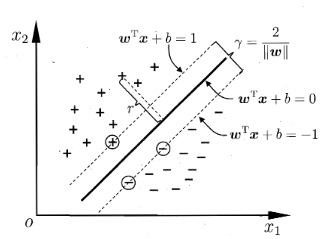
\includegraphics[width=0.309\textwidth]{pic/ML6/间隔与支持向量}
    \caption{间隔与支持向量}
\end{figure}

如图所示, 距离超平面最近的这几个训练样本点使等号成立,它 们 被 称 为 “支持向量”(support vector),两个异类支持向量到超平面的距离之和被 称 为 “间隔”(margin), 为
\begin{align*}
    \gamma=\frac{2}{\norm{\bw}}
\end{align*}

最大间隔: 寻找 $\bw,b$, 使 $\gamma$ 最大. 
\begin{align*}
    &\max_{\bw,b}\frac{2}{\norm{\bw}}\\
    \st& y_i(\bw^\top \bx_i+b)\ge 1,i=1,2,\dots,m
\end{align*}
等价于
\begin{align*}
    &\min_{\bw,b}\frac{1}{2}\norm{\bw}^2\\
    \st& y_i(\bw^\top \bx_i+b)\ge 1,i=1,2,\dots,m
\end{align*}
这就是支持向量机(Support Vector Machine,简 称 SVM ) 的基本型.

\subsection{对偶问题}
用拉格朗日乘子法可得到其“对偶问题”(dual problem). 
\begin{enumerate}
    \item 引入拉格朗日乘子 $a_i\ge 0$ 得到拉格朗日函数
    \begin{align*}
        L(\bw, b, \bm \alpha)=\frac{1}{2}\norm{\bw}^2+\sum_{i=1}^m\alpha_i\left( 1-y_i\left( \bw^\top \bx_i+b \right) \right)
    \end{align*}
    其中 $\bm\alpha = (\alpha_1;\alpha_2;\dots;\alpha_m)$
    \item 令 $L(\bw, b, \bm \alpha)$ 对 $\bw, b$ 的偏导为0
    \begin{align*}
        \bw &= \sum_{i=1}^m\alpha_i y_i\bx_i \\
        0&=\sum_{i=1}^m\alpha_i y_i
    \end{align*}
    \item 回代
    \begin{align*}
        &\max_{\bm\alpha}\sum_{i=1}^m\alpha_i-\frac{1}{2}\left( \sum_{i=1}^m \alpha_i y_i\bx_i^\top\right)\left( \sum_{j=1}^m \alpha_j y_j\bx_j \right)\\
        \st&\sum_{i=1}^m\alpha_i y_i=0, \alpha_i\ge0, i=1,2,\dots,m
    \end{align*}
    这个优化问题可以使用 SMO 方法求解. 
\end{enumerate}
最终模型:
\begin{align*}
    f(\bx)=\bw^\top\bx+b=\sum_{i=1}^m\alpha_iy_i\bx_i^\top\bx+b
\end{align*}

因为有不等式约束, 所以需要满足 KKT 条件, 即
\begin{align*}
    \left\{ \begin{array}{l}
        \alpha_i\ge0\\
        y_if(\bx_i)-1\ge0\\
        \alpha(y_if(\bx_i)-1)=0
    \end{array} \right.
\end{align*}
支持向量机解的稀疏性: 训练完成后,大部分的训练样本都不需保留,最终模型仅与支持向量有关

\subsubsection{SMO 方法}% 最后求解一般都是硬求
不断执行如下两个步骤直至收敛:
\begin{enumerate}
    \item 取一对需更新的变量$\alpha_i,\alpha_j$
    \item 固定 $\alpha_i,\alpha_j$ 以外的参数, 求解优化问题获得更新后的$\alpha_i,\alpha_j$.
\end{enumerate}

仅考虑 $\alpha_i$ 与 $\alpha_j$ 时, 对偶问题约束变为
\begin{align*}
    \alpha_iy_i+\alpha_jy_j=-\sum_{k\ne i,j}a_ky_k, \alpha_i\ge0, \alpha_j\ge 0
\end{align*}
用一个变量表示另一个变量, 回代入对偶问题可. 得一个单变量的二次规划, 该问题具有闭式解.

偏移项 $b$:通过支持向量来确定


\subsection{核函数}
若不存在一个能正确划分两类样本的超平面, 则将样本从原始空间映射到一个更高维的特征空间, 使得样本在这个特征空间内线性可分.

\begin{figure}[!htb]
    \centering
    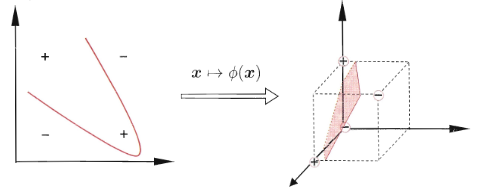
\includegraphics[width=0.42\textwidth]{pic/ML6/异或问题与非线性映射}
    \caption{异或问题与非线性映射}
\end{figure}

令 $\phi(\bx)$ 表示将 $\bx$ 映射后的特征向量, 划分超平面为 $f(\bx)=\bw^\top \phi(\bx)+b$. 

原始问题:
\begin{align*}
    &\min_{\bw,b}\frac{1}{2}\norm{\bw}^2\\
    \st& y_i(\bw^\top \phi(\bx_i)+b)\ge 1,i=1,2,\dots,m
\end{align*}

对偶问题:
\begin{align*}
    &\min_{\bm\alpha}\frac{1}{2}\left( \sum_{i=1}^m \alpha_i y_i\phi(\bx_i)^\top\right)\left( \sum_{j=1}^m \alpha_j y_j\phi(\bx_j) \right)-\sum_{i=1}^m\alpha_i\\
    \st&\sum_{i=1}^m\alpha_i y_i=0, \alpha_i\ge0, i=1,2,\dots,m
\end{align*}

预测:
\begin{align*}
    f(\bx)=\bw^\top\phi(\bx)+b=\sum_{i=1}^m\alpha_iy_i\phi(\bx_i)^\top\phi(\bx)+b
\end{align*}

不显示设计核映射, 而是设计核函数
\begin{align*}
    \kappa(\bx_i, \bx_j)=\phi(\bx_i)^\top \phi(\bx_j)
\end{align*}
\begin{theorem}[Mercer]
    只要一个对称函数所对应的核矩阵半正定,.它就能作为核函数使用 .
\end{theorem}

\begin{figure}[!htb]
    \centering
    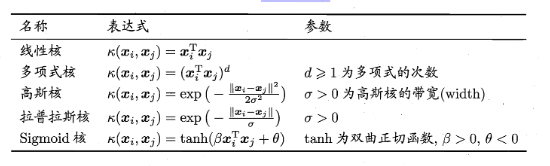
\includegraphics[width=0.42\textwidth]{pic/ML6/常用核函数}
    \caption{常用核函数}
\end{figure}


\subsection{软间隔与正则化}
\subsubsection{软间隔}
在现实任务中往往很难确定合适的核函数使得训练样本在特征空间中线性可分, 同时一个线性可分的结果也很难断定是否是有过拟合造成的.

\begin{figure}[!htb]
    \centering
    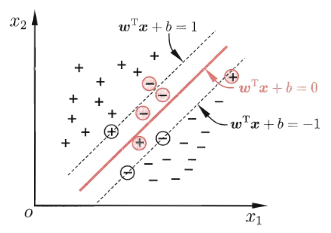
\includegraphics[width=0.309\textwidth]{pic/ML6/软间隔示意图}
    \caption{软间隔示意图}
\end{figure}
引入”软间隔”的概念, 允许支持向量机在一些样本上不满足约束.

基本想法:最大化间隔的同时, 让不满足约束的样本应尽可能少
\begin{align*}
    \min_{\bw, b}\frac{1}{2}\norm{\bw}^2+C\sum_{i=1}^m\ell_{0/1}\left( y_i\left( \bw^\top \bx_i+b \right)-1 \right)
\end{align*}
其中 $C>0$ 为常数, $\ell_{0/1}$ 是 0/1 损失函数
\begin{align*}
    \ell_{0/1}(z)=\left\{ \begin{array}{ll}
        1 & \text{ if }z<0\\
        0 &\text{ otherwise}
    \end{array} \right.
\end{align*}
但其非凸, 非连续. 

于是替代损失函数, 就是软间隔支持向量机, 引入松弛变量 $\zeta_i\ge 0$, 有

原始问题:
\begin{align*}
    &\min_{\bw,b}\frac{1}{2}\norm{\bw}^2+C\sum_{i=1}^m\zeta_i\\
    \st& y_i(\bw^\top \phi(\bx_i)+b)\ge 1-\zeta_i, \zeta_i\ge 0,i=1,2,\dots,m
\end{align*}

对偶问题:
\begin{align*}
    &\min_{\bm\alpha}\frac{1}{2}\left( \sum_{i=1}^m \alpha_i y_i\phi(\bx_i)^\top\right)\left( \sum_{j=1}^m \alpha_j y_j\phi(\bx_j) \right)-\sum_{i=1}^m\alpha_i\\
    \st&\sum_{i=1}^m\alpha_i y_i=0, 0\le \alpha_i\le C, i=1,2,\dots,m
\end{align*}

预测:
\begin{align*}
    f(\bx)=\bw^\top\phi(\bx)+b=\sum_{i=1}^m\alpha_iy_i\phi(\bx_i)^\top\phi(\bx)+b
\end{align*}

\begin{figure}[!htb]
    \centering
    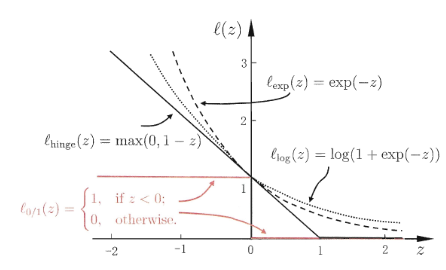
\includegraphics[width=0.309\textwidth]{pic/ML6/三种常见的替代损失函数}
    \caption{三种常见的替代损失函数: hinge损 失 、指数损失、对率损失}
\end{figure}

软间隔支持向量机的最终模型仅与支持向量有关,即通过采用hinge损失函数仍保持了稀疏性. 



\subsubsection{正则化}
支持向量机学习模型的更一般形式
\begin{align*}
    \min_f\Omega(f)+C\sum_{i=1}^m\ell(f(\bx_i), y_i)
\end{align*}
其中, $\Omega(f)$ 称为结构风险, 也称正则化项, 用于描述模型$f$的某些性质; $\ell(f(\bx_i), y_i)$ 称为经验风险, 用于描述模型与训练数据的契合程度. $C$ 用于对二者进行折中, 也称正则化常数. 

正则化是对复杂性的惩罚. 

\subsection{支持向量回归}
允许模型输出和实际输出间存在 $2\epsilon$ 的偏差.
\begin{figure}[!htb]
    \centering
    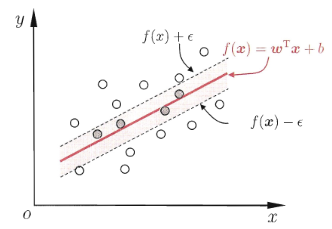
\includegraphics[width=0.309\textwidth]{pic/ML6/支持向量回归示意图}
    \caption{支持向量回归示意图}
\end{figure}

落入中间 $2\epsilon$ 间隔带的样本不计算损失, 从而使得模型获得稀疏性.

\begin{figure}[!htb]
    \centering
    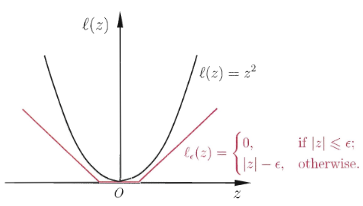
\includegraphics[width=0.42\textwidth]{pic/ML6/不敏感损失函数}
    \caption{$\epsilon$-不敏感损失函数}
\end{figure}

SVR 问题可形式化, 引入 松弛变量 $\zeta_i, \hat{\zeta}_i$

原始问题:
\begin{align*}
    &\min_{\bw,b}\frac{1}{2}\norm{\bw}^2+C\sum_{i=1}^m(\zeta_i-\hat{\zeta}_i)\\
    \st& f(\bx_i)-y_i\le \epsilon+\zeta_i\\
    &y_i-f(\bx_i)\le \epsilon+\zeta_i\\
    &\zeta_i\ge0, \hat{\zeta}_i\ge0,i=1,2,\dots,m
\end{align*}

预测:
\begin{align*}
    f(\bx)=\sum_{i=1}^m(\hat{\alpha}_i-\alpha_i)y_i\bx_i^\top\bx+b
\end{align*}

\subsection{核方法}
\begin{theorem}[表示定理]
    令 $\mathbb{H}$ 为核函数 $\kappa$ 对应的再生核希尔伯特空间, $\norm{h}_{\mathbb{H}}$ 表示 $\mathbb{H}$ 空间中国关于 $h$ 的范数, 对于任意单调递增函数 $\Omega:[0,\infty]\mapsto \R$ 和任意非负损失函数 $\ell : \R^m\mapsto [0,\infty]$, 优化问题
    \begin{align*}
        \min_{h\in\mathbb{H}} F(h)=\Omega(\norm{h}_{\mathbb{H}})+\ell(h(\bx_1), h(\bx_2),\dots,h(\bx_m))
    \end{align*}
    的解总可以写为
    \begin{align*}
        h^*(\bx)=\sum_{i=1}^m\alpha_i\kappa(\bx,\bx_i)
    \end{align*}
\end{theorem}


